\chapter{WP2: Artificial Lagrange Points}
\label{chapter:wp2}

\section{Task 2.1a}

\begin{table}[H]
  \centering
  \caption{Required lightness number to achieve the specified Lagrange point shift.}
  \label{tab:wp2_lagrange_shift}
  \begin{tabular}{@{} l S[table-format=1.5] S[table-format=1.5] @{}}
    \toprule
     & {Shift along Sun-planet line} & {Lightness number, $\beta$} \\
    \midrule
    Sun-Earth - $L_2$ & 0.00100 & 0.01008 \\
    Sun-Mars  - $L_2$ & 0.00100 & 0.01163 \\
    \bottomrule
  \end{tabular}
\end{table}

The highest required $\beta = 0.01163$ (from \autoref{tab:wp2_lagrange_shift}) exceeds lightness numbers of all flown missions \parencite{ancona2024recent}, which reach up to $\beta \approx 0.010$--$0.011$. 
However, Sunjammer \parencite{heiligers2014sunjammer} was designed for comparable performance and passed ground-deployment testing before programmatic cancellation, demonstrating near-term technological feasibility.

% \begin{figure}[H]
%     \centering
%     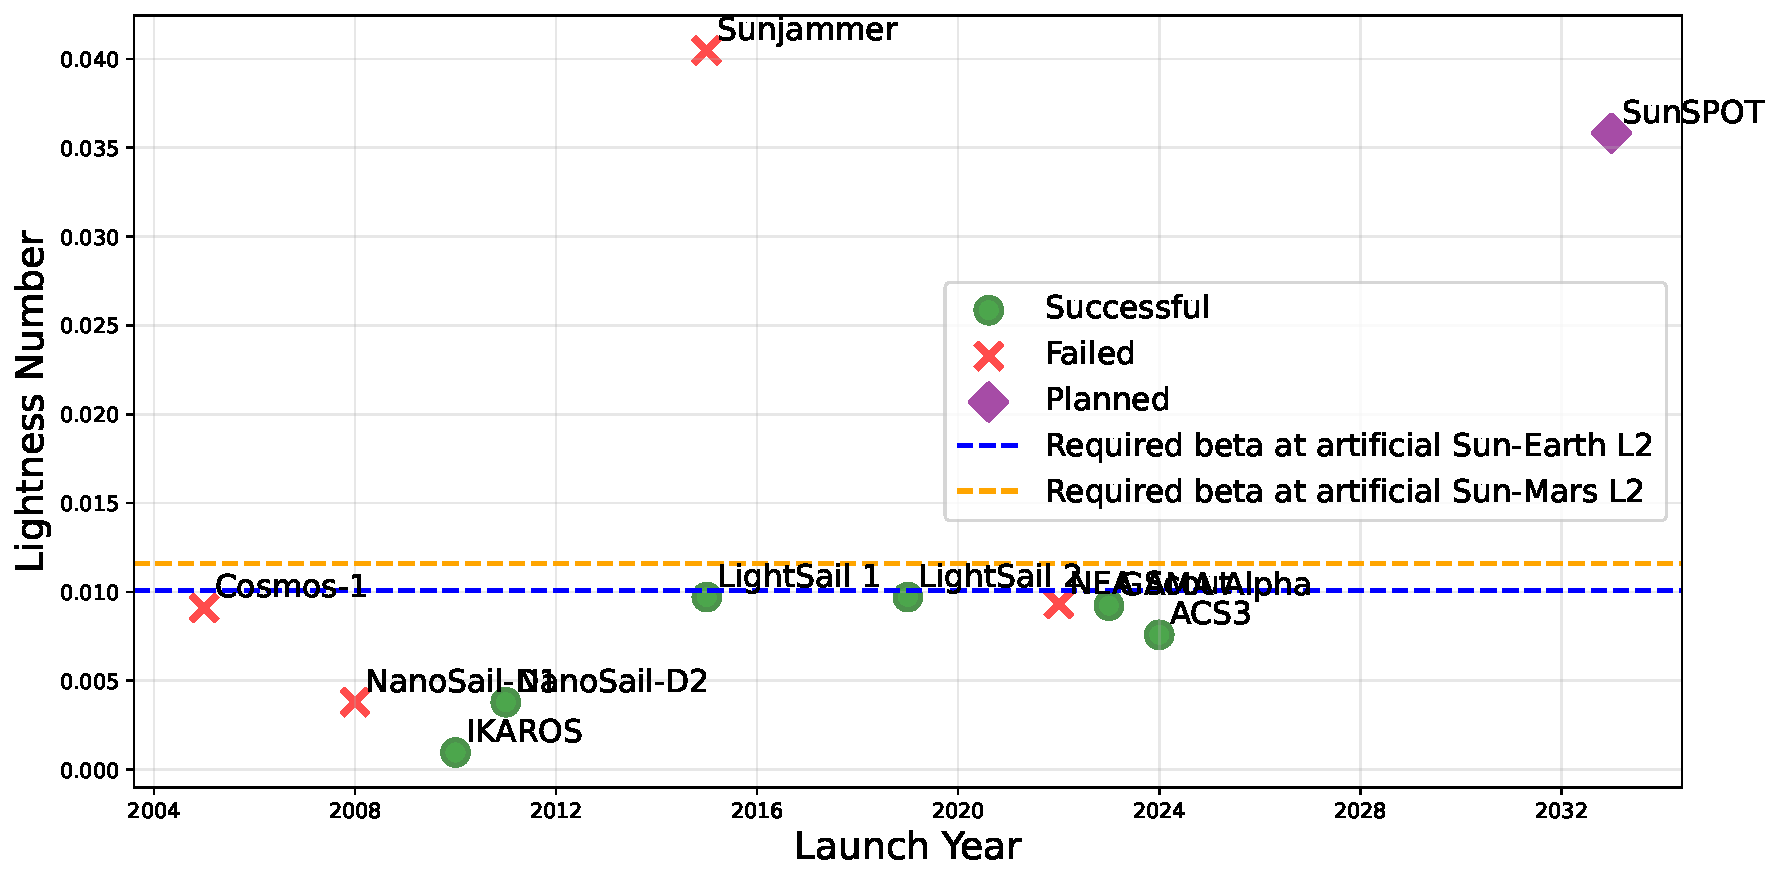
\includegraphics[width=0.8\textwidth]{../code/wps/figures/solar_sail_lightness_number.pdf}
%     \caption{Lightness number of past solar sail missions as a function of their launch year, with the required lightness number for the L2 shift required for each case.}
%     \label{fig:wp2_beta_comparison}
% \end{figure}

(41 words)

\section{Task 2.1b}

\begin{table}[H]
  \centering
  \caption{Required sail orientation to achieve the required shift in the Lagrange points of Task 2.1a.}
  \label{tab:sail_orientation}
  \begin{tabular}{@{} l c c c @{}}
    \toprule
     & $n_{x,i}$ & $n_{y,i}$ & $n_{z,i}$ \\
    \midrule
    Sun-Earth - $L_2$ & 1 & 0 & 0 \\
    Sun-Mars  - $L_2$ & 1 & 0 & 0 \\
    \bottomrule
  \end{tabular}
\end{table}

Apart from the acceleration components in \ref{sec:1.2}, the \acs{srp} acceleration is included, yielding the following expression in the rotating frame:
\begin{equation}
  \mathbf{\ddot{r}} = -2 \mathbf{\omega} \times \mathbf{\dot{r}} - \nabla U + \mathbf{a}_{\text{s}} \xRightarrow{\text{equilibrium}} 0 = -\nabla U + \mathbf{a}_{\text{s}} \Rightarrow \mathbf{a}_{\text{s}} = \nabla U,
\end{equation}
where $\mathbf{a}_{\text{s}}$ is the \acs{srp} solar-sail acceleration, expressed as
\begin{equation}
  \mathbf{a}_{\text{s}} = \beta \frac{1 - \mu}{r^2} (\mathbf{\hat{r}_1} \cdot \mathbf{\hat{n}})^2 \mathbf{\hat{n}}.
\end{equation}
Equilibrium requires $\mathbf{a}_{\text{s}} \parallel \nabla U$, meaning $\mathbf{\hat{n}}$ must be parallel to $\nabla U$. 
For an L2 shift towards the Sun, $\nabla U$ is parallel to the Sun-planet line, so the sail normal must satisfy $\mathbf{\hat{n}} \parallel x$, i.e.\ the sail is oriented perpendicular to that line.

(75 words)

\begin{figure}[H]
  \centering
  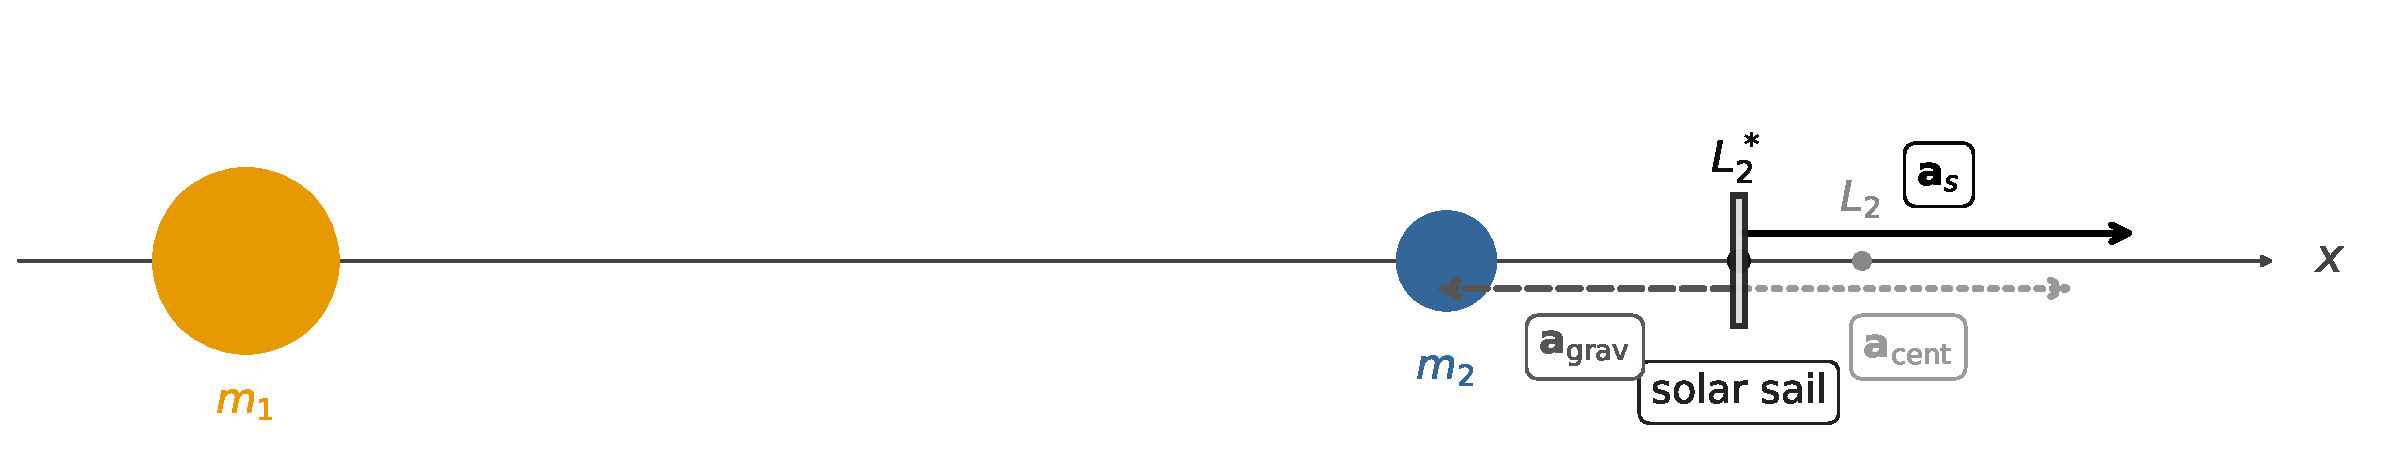
\includegraphics[width=\textwidth]{../code/wps/figures/sail_L2_schematic.pdf}
  \caption{Schematic of all acceleration vectors acting in the solar-sail augmented \ac{cr3bp}.}
  \label{fig:wp2_accel_schematic}
\end{figure}

\section{Task 2.2}
The expressions for the required $\beta$ and sail orientation are analytically derived by \textcite[217]{mcinnes1999book}. 
The validated numerical result for the lightness number is a little bit more complex, as most of the references do not tackle the exact same problem. 
However, from the values in \cite[Table~1]{heiligers2014sunjammer}, the results for the shift in L1 match up to the significant figures provided for the mass parameter. 
On a different level, since the normal vector is parallel to the gradient of the potential \parencite[eq. 5.120]{mcinnes1999book}, the required sail orientation is also verified by the fact of gradient orientation being collinear to the sun-planet line shown in \cite[Fig. 3]{mcinnes1994solar}. 

(99 words)



\section{Task 2.3}

\begin{table}[H]
  \centering
  \caption{Required solar-sail side-length to achieve the required shift in the Lagrange points of Task 2.1a.}
  \label{tab:sail_sidelength}
  \begin{tabular}{@{} l S[table-format=6.2] @{}}
    \toprule
    \textbf{Lagrange Point} & {Required solar-sail side-length [m]} \\
    \midrule
    Sun-Earth Lagrange point & 25.772 \\ % Replace with your calculated value
    Sun-Mars Lagrange point  & 27.676 \\ % Replace with your calculated value
    \bottomrule
  \end{tabular}
\end{table}